\documentclass[12pt]{article}
\usepackage{lastpage}
\usepackage{fancyhdr}
\pagestyle{headings}
\pagenumbering{arabic}
\usepackage{array}
\usepackage{float}
\usepackage{graphicx}
\fancyfoot[R]{\thepage}
\renewcommand{\contentsname}{Cuprins}
\usepackage{listings}

\usepackage[unicode]{hyperref} 
\usepackage[useregional]{datetime2}
\newcommand{\mydate}{\DTMdisplaydate{2017}{12}{14}{-1}}
\begin{document}

\begin{titlepage}
\newcommand{\HRule}{\rule{\linewidth}{0.5mm}} 
\center

\textbf{\LARGE   Universitatea Politehnic\u{a} Bucure\c{s}ti} \\[0.7cm] 
\textsc{\Large \hspace{0.2cm} Facultatea de Automatic\u{a} \c{s}i Calculatoare} \\[2cm]
\center
\textsc{\LARGE Analiza Algoritimilor}\\[1.0cm] 

\center
\HRule \\[0.4cm]
{ \huge \bfseries -TEM\u{A}-}\\[0.4cm] 
\HRule \\[1.5cm]
 

\begin{minipage}{0.9\textwidth}
\begin{flushleft} \large
\LARGE{Student:}\\
 \Large \textbf{Nicu\c{t}\u{a} Loredana - Ionela 315 CD Anul II} 
\end{flushleft}
\end{minipage}
~

\vspace{3.0cm}
{\large \mydate}\\[4cm]
\end{titlepage}

%inceput cuprins
\newpage
\pagestyle{empty}

\tableofcontents

\thispagestyle{empty}
\cleardoublepage
\newpage
\pagestyle{headings}
\setcounter{page}{1}

\section{Tema aleas\u{a}}

\textbf{\hspace{7mm} Tema aleas\u{a} este reprezentat\u{a} de subiectul num\u{a}rul 7: Analiza opera\c{t}iilor asociate unor structuri de date avansate}

\section{Structurile de date alese}

\subsection{AVL Tree}

\textbf{\hspace{7mm}Un AVL Tree, este un arbore binar de c\u{a}utare echilibrat, \^{i}n care diferen\c{t}a \^{i}n\u{a}l\c{t}imilor dintre subarborele st\^{a}ng \c{s}i cel drept nu poate fi mai mare dec\^{a}t 1. \hyperlink{page.14}{[1]} }

\textbf{\hspace{7mm} Complexitate timp: O(log n), unde log n repreznt\u{a} \^{i}n\u{a}l\c{t}imea maxim\u{a} a arborelui. }

\textbf{\hspace{7mm} Complexitate spa\c{t}ial\u{a} : O (n), unde n reprezint\u{a} num\u{a}rul de noduri necesare construirii arborelui.}

\subsubsection{Avantajele folosirii unui AVL Tree}

\begin{enumerate}

\item{\textbf{Fa\c{t}\u{a} de un arbore binar ne-echilibrat, la care complexitatea \^{i}n cel mai r\u{a}u caz va fi este O(n), unde n este num\u{a}rul de noduri \c{s}i reprezint\u{a} \^{i}n\u{a}l\c{t}imea maxim\u{a}, arborele AVL are complexitatea O(log n), av\^{a}nd mereu \^{i}n\u{a}l\c{t}imea log n.}}
\item{\textbf{Un arbore AVL ofer\u{a} posibilitatea de a c\u{a}uta cu u\c{s}urin\c{t}\u{a} un element. }}

\end{enumerate}

\subsubsection{Dezavantajele folosirii unui AVL Tree}

\begin{enumerate}

\item{\textbf{Codul pentru implementarea unui astfel de arbore este mult mai complex dec\^{a}t pentru cel al unui arbore binar ne-echilibrat, fiind nevoie s\u{a} se trateze diferite excep\c{t}ii. }}

\item{\textbf{\^{I}n\u{a}l\c{t}imea arborelui fiind log n, aceasta trebuie men\c{t}inut\u{a}, astfel sunt realizate destul de multe rota\c{t}ii, acest lucru f\u{a}c\^{a}nd alocarea unui spa\c{t}iu \^{i}n plus la input-uri mari.} }

\item{\textbf{\c{S}tergerea unui element are costul mai mare. Complexitatea este \^{i}n continuare O(log n) \^{i}ns\u{a} s-ar putea s\u{a} fie necesare rota\c{t}ii ce se vor extinde p\^{a}n\u{a} la r\u{a}d\u{a}cina arborelui. }}
\end{enumerate}

\subsubsection{Utiliz\u{a}ri practice ale structurii AVL Tree}

\textbf{\hspace{7mm}Se va folosi acest tip de structur\u{a} \^{i}n situa\c{t}iile \^{i}n care avem deja un set de date ini\c{t}ial apropae sortat, \c{s}i vor fi ad\u{a}ugate destul de pu\c{t}ine date pe parcurs sau \c{s}terse, astfel nefiind \^{i}n cazul \^{i}n care trebuie s\u{a} se realizeze mai multe rota\c{t}ii (\^{i}n acest caz, va fi utilizat mai bine un alt arbore binar \c{s}i anume arborele Ro\c{s}u \c{s}i Negru). Astfel, vom putea folosi arborele AVL \c{i}n implementarea unui sistem ce re\c{t}ine rutele unui transport \^{i}n comun, de exemplu trenul, nefiind modificate multe rute/ad\u{a}ugate.  }

\subsection{Segment Tree}

\textbf{\hspace{7mm} Un Segment Tree este un arbore binar folosit pentru a stoca intervale sau segmente. Fiecare nod este format din suma elementelor din subarborele st\^{a}ng \c{s}i cele din subarborele drept, iar frunzele sunt elementele vectorului. \hyperlink{page.14}{[2]}}

\textbf{\hspace{7mm} Complexitate timp: O(log n), unde log n repreznt\u{a} \^{i}n\u{a}l\c{t}imea maxim\u{a} a arborelui. }

\textbf{\hspace{7mm} Complexitate spa\c{t}ial\u{a} : O (4 * n), unde 4 * n reprezint\u{a} num\u{a}rul de noduri necesare construirii arborelui (num\u{a}rul de noduri dintr-un arbore binar este de maxim 2 pow( [(log n ) + 1]) , unde log n + 1 reprezint\u{a} \^{i}n\u{a}l\c{t}imea) .}

\subsubsection{Avantajele utiliz\u{a}rii unui Segment Tree}

\begin{enumerate}
\item{\textbf{Este o structur\u{a} flexibil\u{a} ce permite diferite opera\c{t}ii asupra elementelor dintr-un vector. (g\u{a}sirea elementului minim, g\u{a}sirea elementului maxim, calcularea sumei, calcularea celui mai mic divisor comun ...).}}

\item{\textbf{Opera\c{t}iile de ad\u{a}ugare, \c{s}tergere, c\u{a}utare a unui element au complaxitatea O(log n).}}

\end{enumerate}

\subsubsection{Dezvantajele utiliz\u{a}rii unui Segment Tree}

\begin{enumerate}

\item{\textbf{Folosirea de memorie destul de mult\u{a} comporativ cu alte implement\u{a}ri ale arborilor binari. \^{I}n tot arborele, vom avea numai n elemente din vector, restul reprezent\^{a}nd suma dintre acestea. Astfel complexitatea spa\c{t}ial\u{a} va fi de O (4 * n), unde n reprezint\u{a} num\u{a}rul de noduri din vectorul in\c{t}ial. }}

\item{\textbf{Dintr-un Segment Tree nu se pot \c{s}terge propriu-zis elemente, ci vor fi marcate cu un num\u{a}r negativ. O alt\u{a} solu\c{t}ie este crearea unui nou Segment Tree cu noul vector din care a fost eliminat elementul dorit. Aceast\u{a} metoda este extrem de ineficient\u{a}}.}


\end{enumerate}
	

\subsubsection{Utiliz\u{a}ri practice ale structurii Segment Tree}
\textbf{\hspace{7mm} Se va folosi acest tip de structur\u{a} \^{i}n situa\c{t}iile \^{i}n care vom avea un set de date ini\c{t}ial stabilit, asupra c\u{a}ruia nu vom mai dori sa ad\u{a}ug\u{a}m noi elemnte, ci doar s\u{a} le modific\u{a}m valoarea eventual. Fiecare ad\u{a}ugare/\c{s}tergere reprezint\u{a} realizarea unui nou arbore de acest tip, exist\^{a}nd alte structuri mai eficiente \^{i}n acest caz. Astfel, vom putea utiliza aceast\u{a} structur\u{a} atunci c\^{a}nd vom dori s\u{a} realiz\u{a}m pe un set de date, diferite opera\c{t}ii dintr-un anumit interval. (Ex. Calcularea minimului subsirului dat de x si y, Calcularea sumei primelor x elemente dintr-un vector ...). }
\newpage
\section{Analiza opera\c{t}iilor specifice}
\textbf{\hspace{7mm} \^{I}n realizarea acestor teste, am implementat structurile \c{s}i opera\c{t}iile necesare \^{i}n Java. Pentru AVL, codul a fost luat de aici : \href{http://www.geeksforgeeks.org/avl-tree-set-2-deletion/}{[cod]}, iar pentru Segment de aici : \href{https://algs4.cs.princeton.edu/99misc/SegmentTree.java.html}{[cod]}. Pentru testare \c{s}i adaptare, au fost selectate metodele, respectiv ad\u{a}ugate.}
\subsection{Ad\u{a}ugarea elementelor}
\subsubsection{Ad\u{a}ugarea unui element \^{i}ntr-un AVL Tree}
\textbf{\hspace{7mm} Arborele AVL este un arbore echilibrat (avem diferenta \^{i}n\u{a}l\c{t}imilor subarborelui stang, respectiv celui drept de cel mult 1). Astfel, atunci c\^{a}nd un element este inserat \^{i}ntr-un astfel de arbore, se va realiza mereu la final re-echilibrarea arborelui, complaxitatea opera\c{t}iei de ad\u{a}ugare fiind mereu O(log n), unde log n reprezint\u{a} \^{i}n\u{a}l\c{t}imea arborelui AVL.}

\textbf{\hspace{2mm}Re-echilibrarea unui arbore const\u{a} \^{i}n realizarea unor rota\c{t}ii simple sau duble, urmate de recalcularea \^{i}n\u{a}l\c{t}imii fiec\u{a}rui nod \^{i}nt\^{a}lnit parcurg\^{a}nd arborele de jos \^{i}n sus, spre r\u{a}d\u{a}cin\u{a}.}


\textbf{\hspace{2mm}Pa\c{s}ii ce vor fi urm\u{a}ri\c{t}i la inserarea unui elemnt \^{i}ntr-un arbore AVL:}
\begin{enumerate}

\item{\textbf{Se insereaz\u{a} elementul ca \^{i}ntr-un arbore binar ordonat obi\c{s}nuit: se porne\c{s}te de la r\u{a}d\u{a}cin\u{a} \c{s}i se urmeaz\u{a} fiul st\^{a}ng sau fiul drept, \^{i}n func\c{t}ie de rela\c{t}ia dintre cheia de inserat \c{s}i cheia nodurilor prin care se trece.}}

\item{\textbf{Dup\u{a} ce elementul a fost introdus, se se parcurge drumul invers (unic) \c{s}i se caut\u{a} pe acest drum primul nod care nu este echilibrat, adicu{a} primul nod ai c\u{a}rui subarbori difer\u{a} ca \^{i}n\u{a}l\c{t}ime prin 2 unita\c{t}i. Fiecare element ad\u{a}ugat ce necesit\u{a} rota\c{t}ii se va afla \^{i}n unul dintre cazurile ilustrate \^{i}n figur\u{a}. (\hyperlink{page.14}{[3]}).}}

\end{enumerate}
\begin{figure}[H]
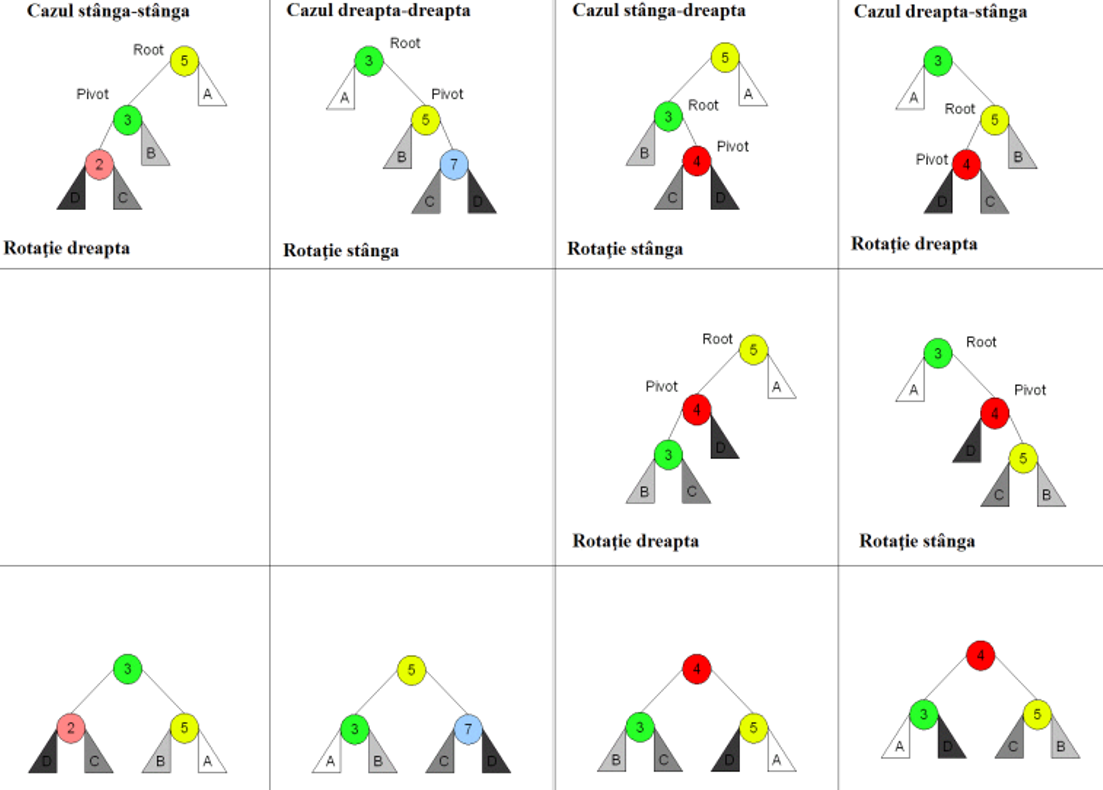
\includegraphics[scale = 0.5]{Rotate.png}
\caption{Cazurile de rota\c{t}ie \^{i}ntr-un arbore AVL}
\label{fig:rotate}
\end{figure}

\subsubsection{Ad\u{a}ugarea unui element \^{i}ntr-un Segment Tree}
\textbf{\hspace{7mm} Arborele Segment este o structur\u{a} de date folosit\u{a} mai ales pentru a stoca informa\c{t}ii despre intervale sau segmente. Aceast\u{a} structur\u{a} nu se poate modifica odata ce a fost creat\u{a}, complaxitatea opera\c{t}ii de ad\u{a}ugare fiind mereu O(log n), unde log n reprezint\u{a} \^{i}n\u{a}l\c{t}imea arborelui AVL. }

\textbf{\hspace{2mm} Pa\c{s}ii ce vor fi urm\u{a}ri\c{t}i la inserarea unui elemnt \^{i}ntr-un arbore Segment:}
\begin{enumerate}
\item{\textbf{Vom ad\u{a}uga mai \^{i}nt\^{a}i toate elementele dorite \^{i}ntr-un vector de dimensiune n. Acesta va repreznta baza construc\c{t}iei arborelui Segment.}}
\item{\textbf{Pentru construirea arborelui, vom \^{i}ncepe cu vectorul [0 ... n - 1] \c{s}i de fiecare dat\u{a} c\^{a}nd \^{i}mp\u{a}r\c{t}im vectorul \^{i}n jum\u{a}tate, vom salva \^{i}n nodul curent ceea ce ne intereseaz\u{a} (suma, minim, maxim, etc.)  \c{s}i continu\u{a}m p\^{a}n\u{a} vectorul va fi de lungime 1. Astfel, vom ajunge s\u{a} avem drept frunze toate elementele vectorului ini\c{t}ial. \hyperlink{page.14}{[4]} }}

\end{enumerate}

\begin{figure}[H]
\centering
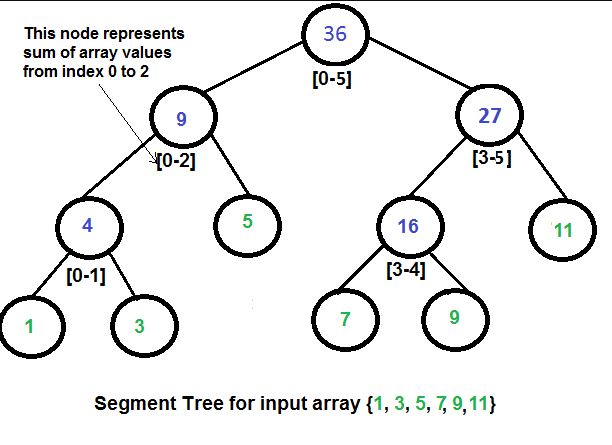
\includegraphics[scale = 0.4]{Rotatii.png}
\caption{Exemplu de inserare \^{i}ntr-un arbore Segment}
\end{figure}

\subsubsection{Testarea implement\u{a}rilor pe diferite teste}

\begin{figure}[H]
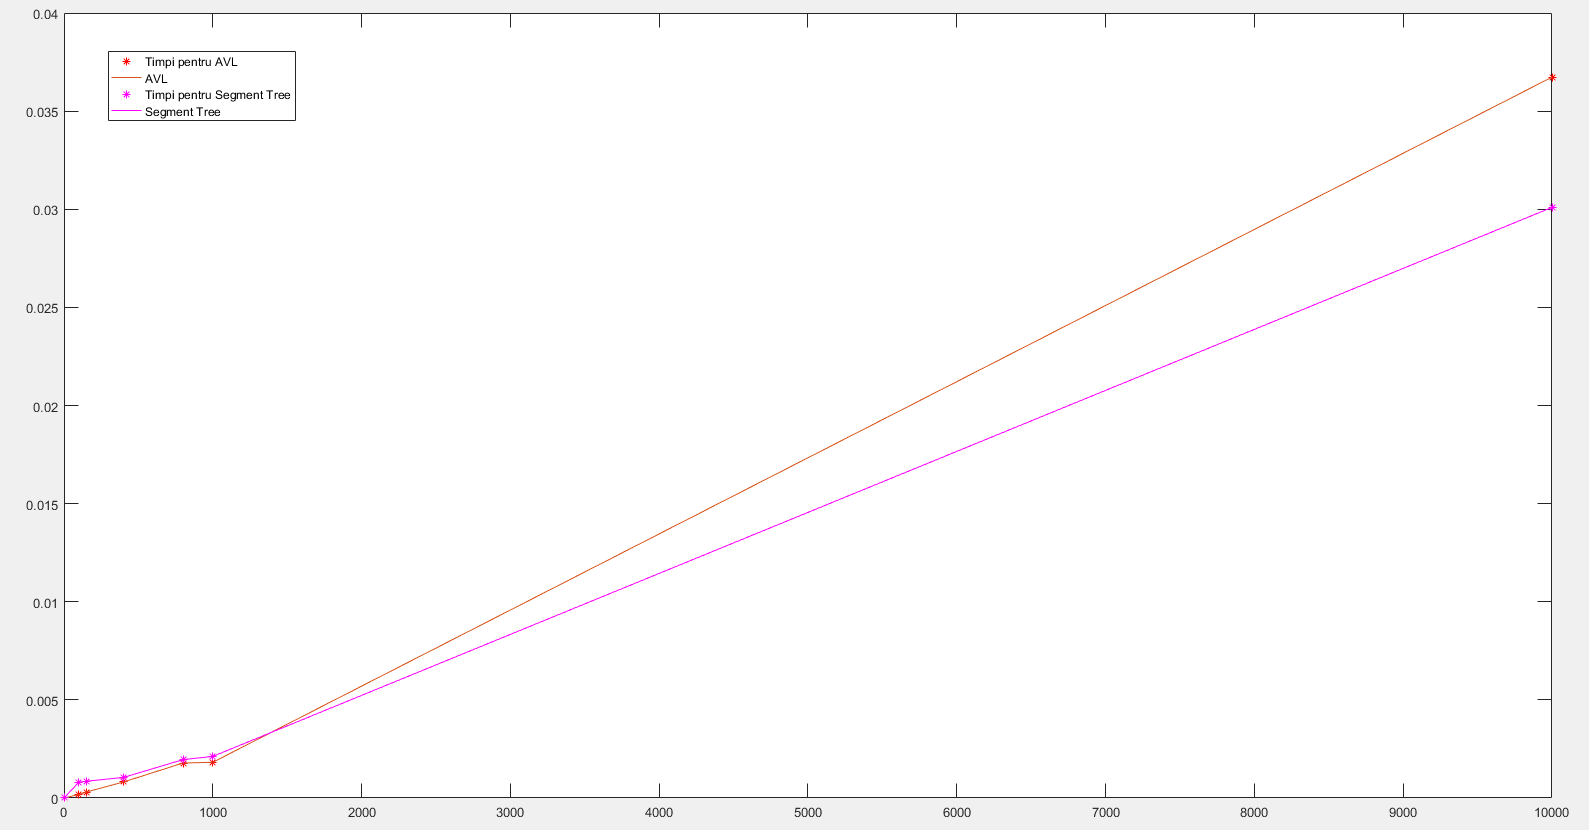
\includegraphics[scale = 0.37]{Insert.png}
\caption{Evolu\c{t}ia temporal\u{a} la inserarea elementelor}
\end{figure}

\textbf{\hspace{7mm} Se observ\u{a} \c{s}i de pe grafic faptul c\u{a} arborele AVL, fa\c{t}\u{a} de arborele Segment este o bun\u{a} implemntare atunci c\^{a}nd avem teste de dimensiuni relativ mici (100 - 1000) de elemente, \^{i}ns\u{a} cu c\^{a}t datele sunt mai multe, cu at\^{a}t dureaz\u{a} mai mult fiind nevoie de multe re-echilibrari. }
\subsection{\c{S}tergerea elementelor}

\subsubsection{\c{S}tergerea elementelor dintr-un AVL Tree}


\textbf{\hspace{7mm} Atunci c\^{a}nd se dore\c{s}te \c{s}trgerea unui element dintr-un AVL Tree, va trebui mai \^{i}nt\^{a}i s\u{a} se caute acel element. \^{I}n cazul \^{i}n care acesta a fost g\u{a}sit se va rupe leg\u{a}tura cu p\u{a}rintele elementului \c{s}i se va realiza o nou\u{a} leg\u{a}tur\u{a} cu poten\c{t}ialii copii al elementului eliminat.}

\textbf{Dup\u{a} ce se \c{s}terge fizic elementul, vom realiza re-echilibrarea arborelui, \^{i}n acela\c{s}i mod \^{i}n care am realizat-o la ad\u{a}ugarea unui element. Aceast\u{a} opera\c{t}ie are complexitatea O(log n), deoarece \^{i}n cel mai r\u{a}u caz, vom avea de parcurs arborele p\^{a}n\u{a} la \^{i}n\u{a}l\c{t}imea maxim\u{a} pentru a g\u{a}si elementul ce se dore\c{s}te a fi \c{s}ters.\hyperlink{page.14}{[5]}}


\subsubsection{\c{S}tergerea elementelor dintr-un Segment Tree}

\textbf{Atunci c\^{a}nd se dore\c{s}te \c{s}tergerea unui element dintr-un Segment Tree, exist\u{a} dou\u{a} posibilit\u{a}\c{t}i de abordare asupra acestei probleme: }

\begin{enumerate}

\item{\textbf{Se caut\u{a} elementul \^{i}n vectorul ini\c{t}ial, se \c{s}terge, iar mai apoi se realizeaz\u{a} un NOU arbore de tip Segment, ce nu va con\c{t}ine elementul \c{s}ters. }}

\item{\textbf{Se caut\u{a} \^{i}n arbore elementul ce se dore\c{s}te a fi \c{s}ters \c{s}i se \^{i}nlocuie\c{s}te cu un num\u{a}r negativ. Aceast\u{a} metod\u{a} se poate folosi atunci c\^{a}nd avem doar numere pozitive \^{i}n cadrul vectorului. }}

\end{enumerate}

\textbf{\hspace{7mm} Aceast\u{a} opera\c{t}ie are complexitatea maxim\u{a} O(log n), unde log n reprezint\u{a} \^{i}n\u{a}l\c{t}imea meaxim\u{a} a arborelui.}
\subsubsection{Testarea implement\u{a}rilor pe diferite teste}

\begin{figure}[H]
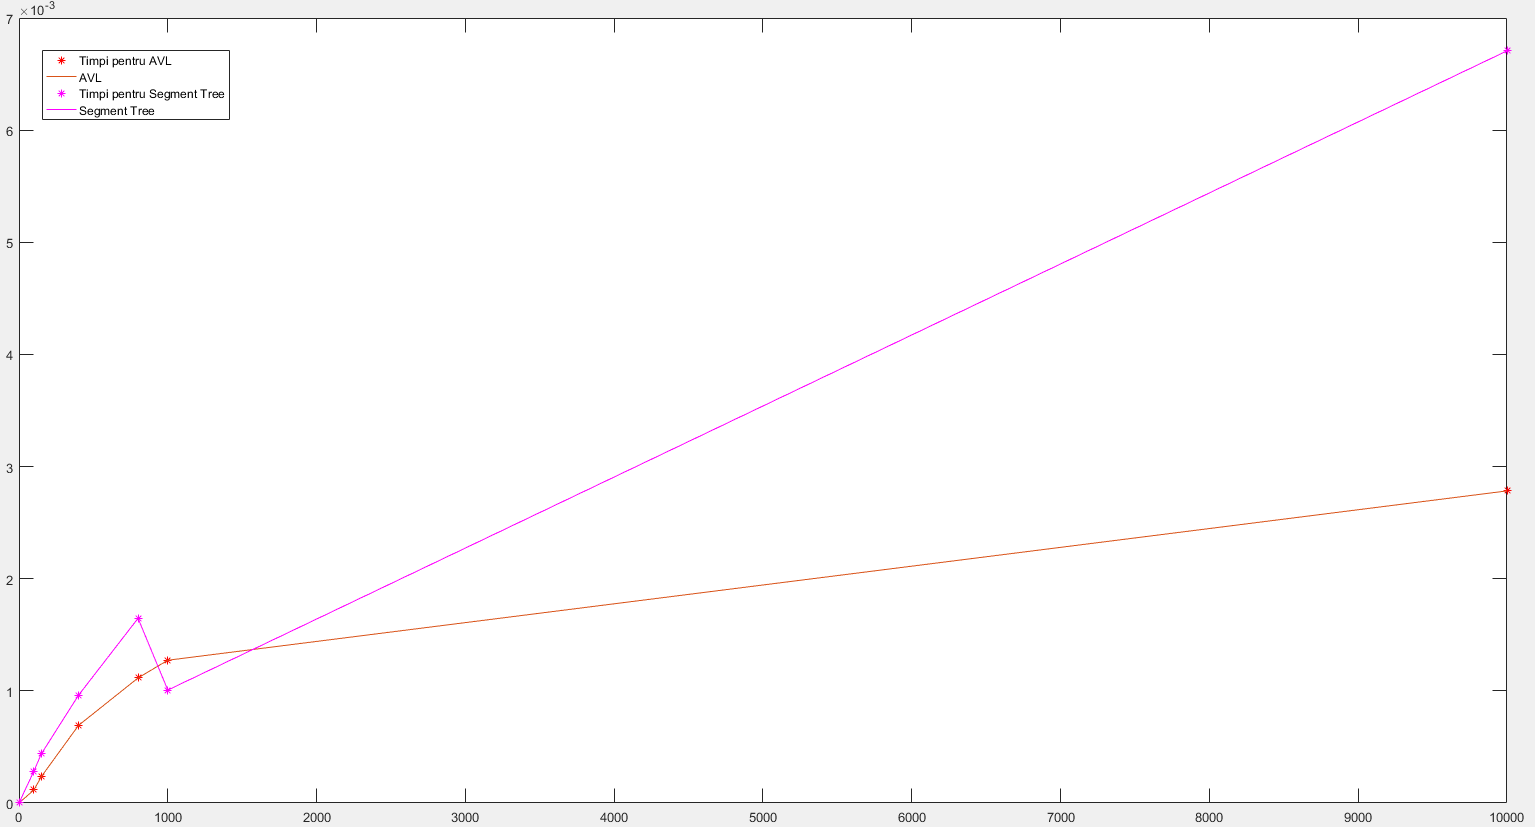
\includegraphics[scale = 0.4]{Delete.png}
\caption{Evolu\c{t}ia temporal\u{a} la \c{s}tergerea elementelor}
\end{figure}
\textbf{\hspace{7mm}Se observ\u{a} \c{s}i de pe grafic faptul c\u{a} atunci c\^{a}nd se vor \c{s}terge elementele din vector, este mult mai eficient arborele AVL. Acest lucru se datoreaz\u{a} \^{i}n primul r\^{a}nd datorit\u{a} complexit\u{a}\c{t}ilor spa\c{t}iale diferite.}

\newpage
\subsection{G\u{a}sirea elementului minim}

\subsubsection{G\u{a}sirea elementului minim \^{i}ntr-un AVL Tree}

\textbf{\hspace{7mm} Pentru a determina minimul din arbore, se va parcurge toat\u{a} structura \^{i}ncep\^{a}nd cu r\u{a}d\u{a}cina \c{s}i se va parcurge c\^{a}t mai la "st\^{a}nga" posibil.}

\begin{figure}[H]
\centering
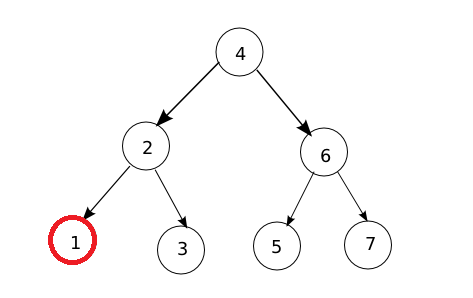
\includegraphics[scale = 0.5]{AvlMin.png}
\caption{Elementul minim \^{i}ntr-un arbore AVL}
\end{figure}

\subsubsection{G\u{a}sirea elementului minim \^{i}ntr-un Segment Tree}

\textbf{\hspace{7mm} Pentru a determina minimul dintr-un anumit interval, se vor alege mai \^{i}nt\^{a}i cele dou\u{a} capete, se va c\u{a}uta \^{i}n arbore zonele unde se g\u{a}sesc acele valori \c{s}i se determin\u{a} minimul frunzelor. ! Se poate optimiza acest task prin p\u{a}strarea \^{i}n nodurile interne, minimul dintre cei doi copii. Aceast\u{a} opera\c{t}ie are complexitatea de O(log n), unde log n reprezint\u{a} \^{i}n\u{a}l\c{t}imea meaxim\u{a} a arborelui. \hyperlink{page.14}{[6]} }

\begin{figure}[H]
\centering
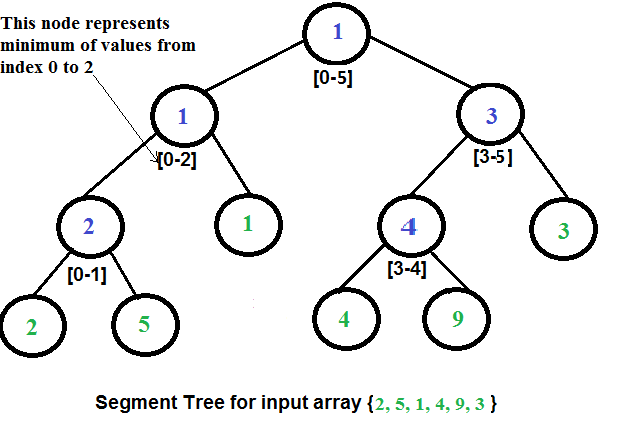
\includegraphics[scale = 0.45]{Minim.png}
\caption{Elementul minim \^{i}ntr-un arbore Segment}
\end{figure}

\subsubsection{Testarea implement\u{a}rilor pe diferite teste}

\begin{figure}[H]
\centering
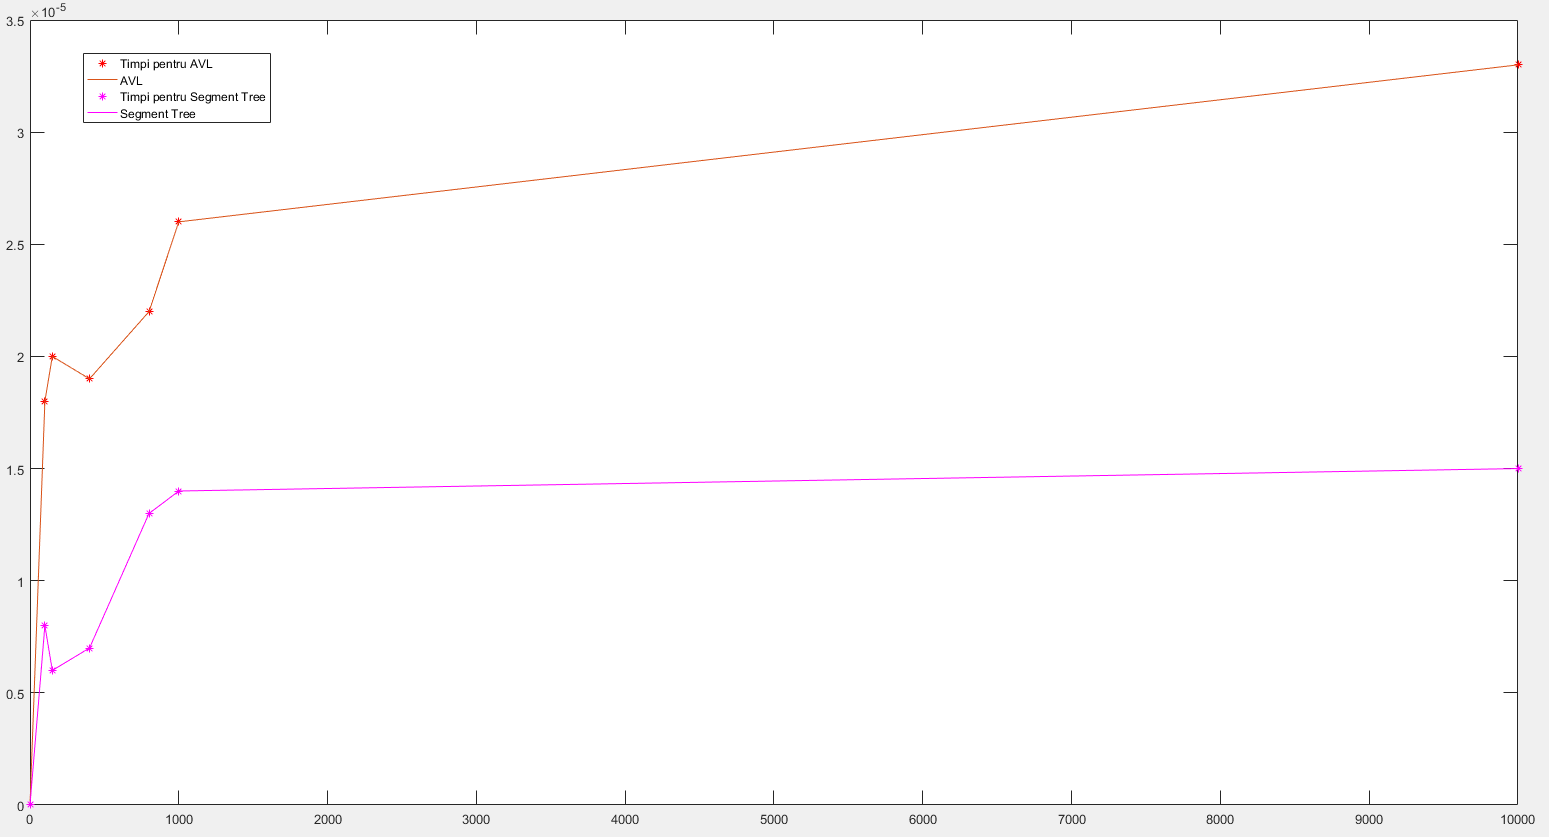
\includegraphics[scale = 0.4]{Min.png}
\caption{Evolu\c{t}ia temporal\u{a} la g\u{a}sirea elementului minim}
\end{figure}

\textbf{\hspace{7mm} Se observ\u{a} \c{s}i de pe grafic faptul c\u{a} atunci c\^{a}nd vine vorba de opera\c{t}ii de tipul c\u{a}utarea minumului, arborele Segment va avea un timp de execu\c{t}ie mult mai bun dec\^{a}t cel al arborelui AVL.}
\subsection{G\u{a}sirea elementelor mai mici dec\^{a}t un element \^{i}ntr-un arbore AVL}

\textbf{\hspace{7mm}Pentru a determina toate elementele mai mici dec\^{a}t un alt element, se va c\u{a}uta prima dat\u{a} elementul \^{i}n arbore, iar dac\u{a} va fi g\u{a}sit se va afi\c{s}a \^{i}ntreg arborele st\^{a}ng. Aceast\u{a} opera\c{t}ie are complexitatea de O(log n), unde log n reprezint\u{a} \^{i}n\u{a}l\c{t}imea maxim\u{a} a arborelui.}

\subsubsection{Testarea implement\u{a}rii pe diferite teste}

\begin{figure}[H]
\centering
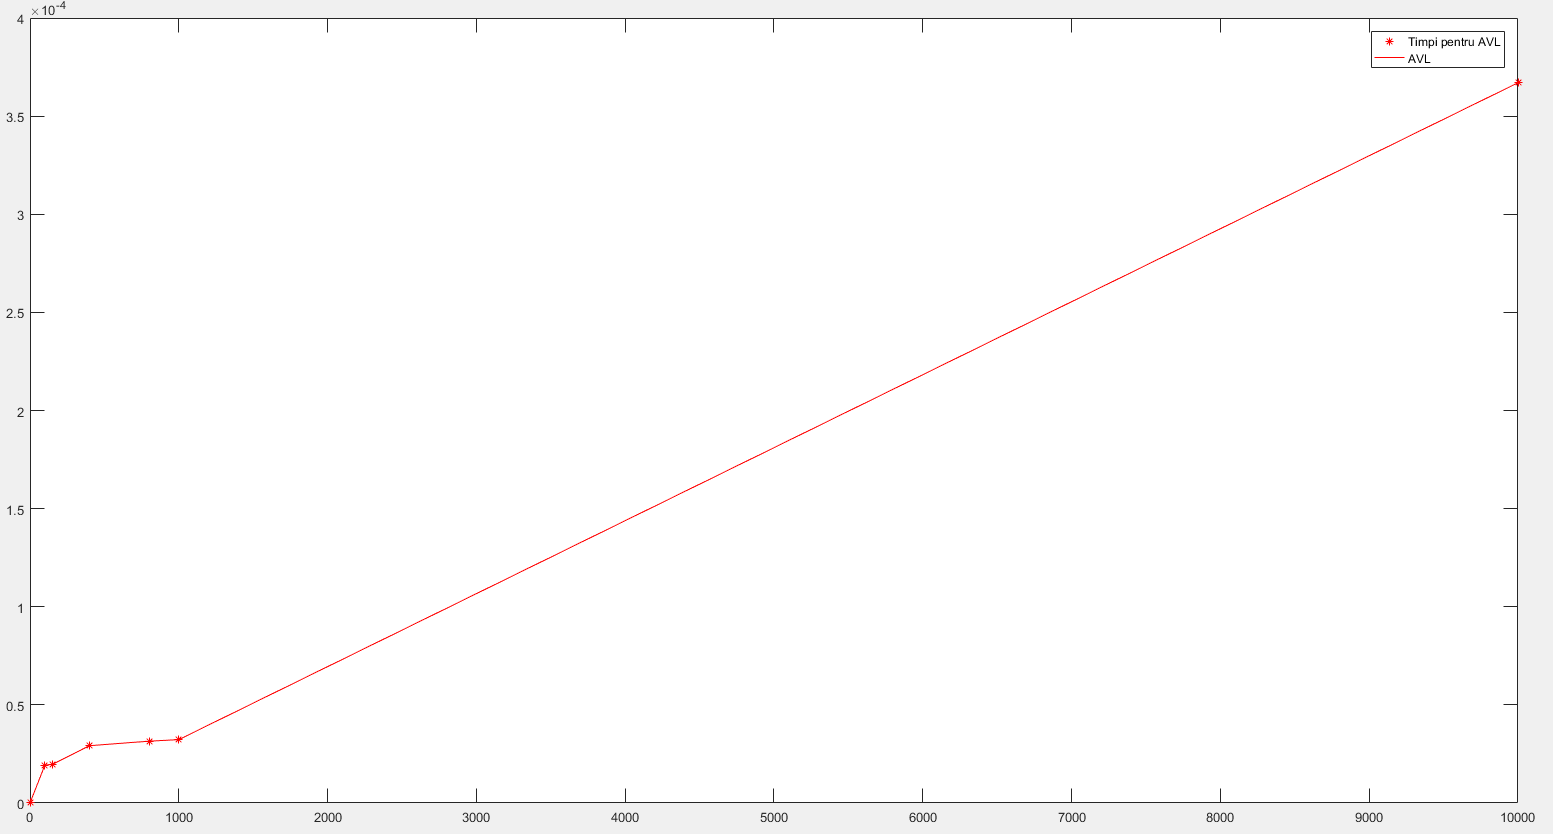
\includegraphics[scale = 0.4]{MinAVL.png}
\caption{Evolu\c{t}ia temporal\u{a} la gasirea elementelor mai mici dec\^{a}t un element dat \^{i}ntr-un AVL Tree}
\end{figure}	

\subsection{\^{I}nlocuirea unui element x cu y \^{i}ntr-un arbore Segment}	
\textbf{\hspace{7mm} Pentru a putea \^{i}nlocui un element dintr-un arbore Segment, se va parcurge lista de elemente, se va salva indexul elementului \c{s}i se va parcurge arborele p\^{a}n\u{a} se va ajunge la intervalul de tip [index, index], \^{i}nlocuidu-se valoarea ini\c{t}ial\u{a} cu cea final\u{a}. Aceasta\u{a} opera\c{t}ie are complexitatea de O(log n), unde log n reprezint\u{a} \^{i}n\u{a}l\c{t}imea maxim\u{a} a arborelui. \hyperlink{page.14}{[2]}}

\subsubsection{Testarea implement\u{a}rilor pe diferite teste}

\begin{figure}[H]
\centering
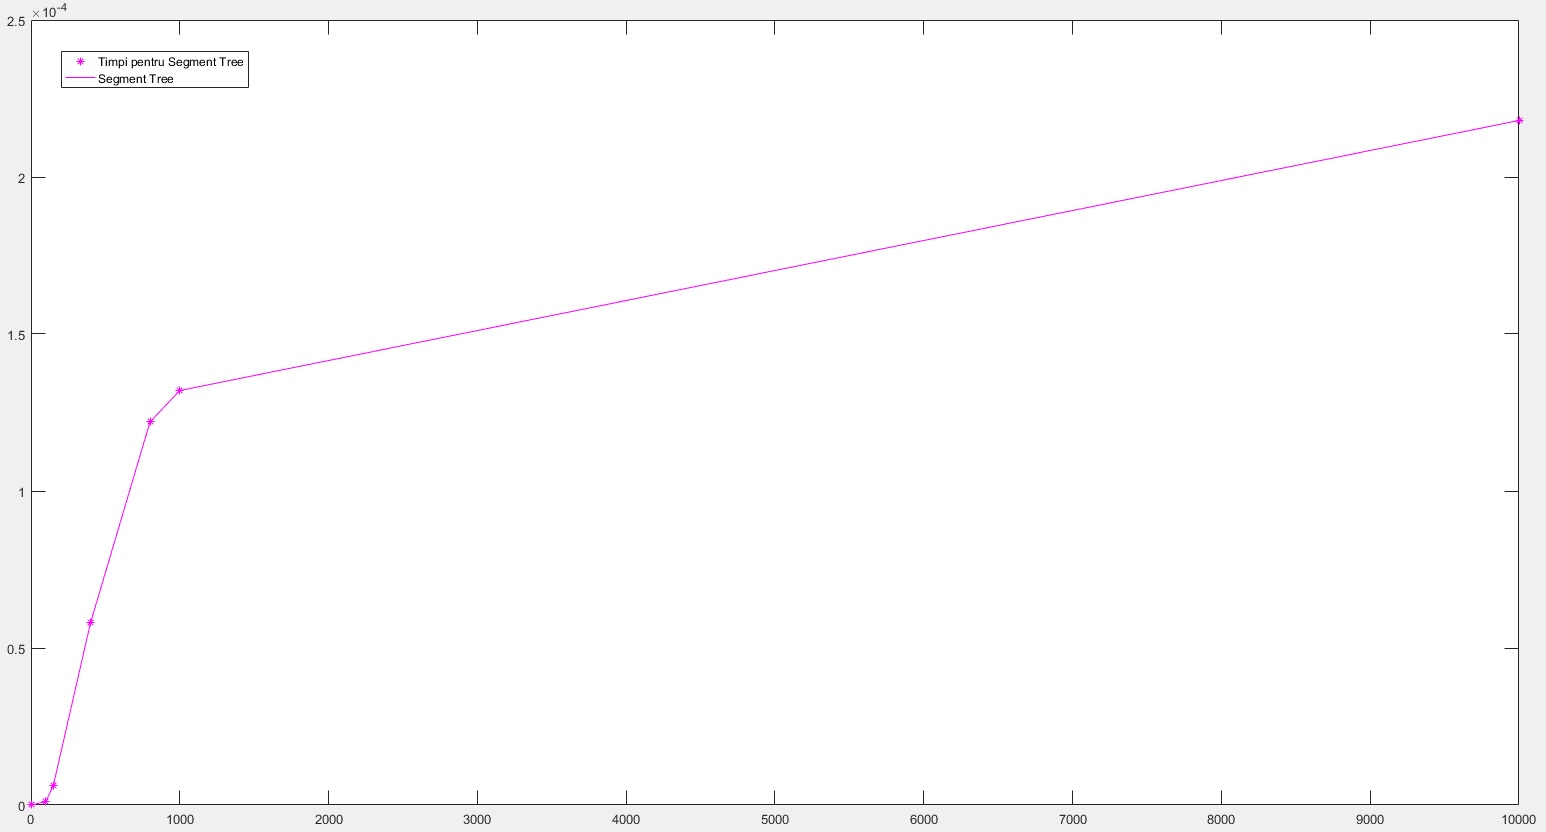
\includegraphics[scale = 0.4]{ReplaceSeg.png}
\caption{Evolu\c{t}ia temporal\u{a} la \^{i}nlocuirea unui element existent \^{i}ntr-un arbore Segment}
\end{figure}

\newpage
\section{Concluzie}
\textbf{\hspace{7mm} At\^{a}t arborele AVL, c\^{a}t \c{s}i arborele Segment sunt dou\u{a} structuri de date avansate, ce au scopul de a facilita \c{s}i de a \^{i}mbun\u{a}t\u{a}\c{t}i modalitatea de rezolvarea a problemelor. Dup\u{a} cum s-a observat \^{i}n graficele de mai sus, fiecare structur\u{a} are un comportament diferit, ce poate fi, sau nu, benefic \^{i}n anumite situa\c{t}ii.}

\textbf{\hspace{2mm} Arborele AVL are timpi de execu\c{t}ie asupra ad\u{a}ug\u{a}rii elementelor, respectiv asupra determin\u{a}rii minimului, mai mari, \^{i}ns\u{a} atunci c\^{a}nd avem un set de date asupra c\u{a}ruia nu dorim s\u{a} realiz\u{a}m alte oper\c{t}ii \^{i}n afar\u{a} de cele declarate mai sus, este o structur\u{a} u\c{s}or de \^{i}n\c{t}eles, respectiv accesibil\u{a}.}

\textbf{\hspace{2mm} Arborele Segment are timpi de execu\c{t}ie mai slabi la "\c{s}tergere", respectiv la ad\u{a}ugarea elementelor, pe teste de dimensiuni mai mari ($ > 1000$) , \^{i}ns\u{a} atunci c\^{a}nd avem opera\c{t}ii de procesare a elementelor, arborele Segment este o variant\u{a} mult mai bun\u{a}.}
\newpage
\section{Bibliografie}
\hspace{5mm} \href{https://en.wikipedia.org/wiki/AVL_tree}{[1]. Detalii AVL}

\href{https://en.wikipedia.org/wiki/Segment_tree}{[2]. Detalii Segment Tree}

\href{http://www.geeksforgeeks.org/avl-tree-set-1-insertion/}{[3]. Explica\c{t}ii contruire arbore AVL}

\href{http://www.geeksforgeeks.org/segment-tree-set-1-sum-of-given-range/}{[4]. Explica\c{t}ii contruire arbore Segment}

\href{http://www.geeksforgeeks.org/avl-tree-set-2-deletion/}{[5]. Explica\c{t}ii pentru \c{s}tergerea elementelor dintr-un arbore AVL}

\href{http://www.geeksforgeeks.org/segment-tree-set-1-range-minimum-query/} {[6]. Explica\c{t}ii pentru calcularea minimului \^{i}ntr-un arbore Segment}


\end{document}